\section{System STLC-Impure}

This chapter describes an extension of system STLC-Pure, where there
exists both effect-disciplined functions (stoic functions) and
effect-arbitrary functions (free functions). As there's a
subtyping between the two kinds of functions, it's natural to
integrate subtyping in the system.

We'll first introduce the formalization, then discuss soundness and
effect safety. In the discussion, we'll focus on its difference from
system STLC-Pure.

\subsection{Definitions}

Initially, we arrived at a formualtion of the system shown in
Figure~\ref{fig:stlc-impure-definition-first}. It's a straight-forward
extension of SLTC-Pure with subtyping and free functions. Note
that in this formulation, we need to change the definition of the
\emph{pure} function to exclude free function types in the pure
environment. This restriction is important, because we're not sure
what side effects there might be inside free functions. If we
allow stoic functions have access to free functions, we'll loose
the ability to track the effects of stoic functions in the type
system.

The definition is all good, except that perservation breaks! The
problem is caused by using an impure term as \emph{Top}. To see a
concrete example, let's assume $\Gamma = \{c:E\}$. It's obvious that
following term is well-typed under $\Gamma$ as $B \to Top$:

\begin{center}
  $(\lambda x:Top. \; \lambda y:B. \; x) \; c$
\end{center}

However, after one evaluation step\footnote{Note that variables are
  values, thus we can take a step here. We can also construct a
  counter-example by wrap $c$ in a lambda abstraction like
  $\lambda x:B. c$.}, we get the term $\lambda y:B. \; c$, which can
at best be typed as $B \Rightarrow Top$. Thus preservation doesn't
hold in current formulation. This problem leads us to two different
formuations.

\begin{figure}
\begin{framed}

% multi-column separator
\setlength{\columnseprule}{0.4pt}
\begin{multicols}{2}

\textbf{Syntax}

\begin{tabu} to \linewidth {l l l X[r]}
  t   & ::= &                    & terms:               \\
      &     &  x                 & variable             \\
      &     & $\lambda$ x:T.t    & abstraction          \\
      &     & t t                & application          \\
\\
  v   & ::= &                    & values:              \\
      &     & $\lambda$ x:T.t    & abstraction value    \\
      &     & x                  & variable value       \\
\\
  T   & ::= &                    & types:               \\
      &     & \colorbox{shade}{Top}  & top type             \\
      &     & B                  & basic type           \\
      &     & E                  & capability type      \\
      &     & T $\to$ T          & type of stoic funs       \\
      &     & \colorbox{shade}{T $\Rightarrow$ T} & type of free funs   \\
\end{tabu}

\hfill\\

\textbf{Evaluation} \hfill \framebox[1.2\width][r]{$t \longrightarrow t'$}

\infrule[E-App1]
{ t_1 \longrightarrow t'_1 }
{ t_1 \; t_2 \longrightarrow t'_1 \; t_2 }

\infrule[E-App2]
{ t_2 \longrightarrow t'_2 }
{ v_1 \; t_2 \longrightarrow v_1 \; t'_2 }

\infax[E-AppAbs]
{ (\lambda x:T.t_1) v_2 \longrightarrow [x \mapsto v_2]t_1 }

\textbf{Pure Environment}

\begin{center}
\begin{tabular}{l c l}
pure($\varnothing$)                   & = &   $\varnothing$ \\
pure($\Gamma$, x: E)                  & = &  pure($\Gamma$) \\
\rowcolor{gray!40}
pure($\Gamma$, x: S $\Rightarrow$ T)  & = &  pure($\Gamma$) \\
pure($\Gamma$, x: T)                  & = &  pure($\Gamma$), x: T     \\
\end{tabular}
\end{center}

\columnbreak

\textbf{Typing}  \hfill \framebox[1.2\width][r]{$\Gamma \vdash x : T$}

\infrule[T-Var]
{ x: T \in \Gamma }
{ \Gamma \vdash x : T }

\infrule[T-Abs1]
{ pure(\Gamma),\; x: S \vdash t_2 : T }
{ \Gamma \vdash \lambda x:S.t_2 : S \to T }

\infrule[T-Abs2]
{  \colorbox{shade}{$\Gamma,\; x: S \vdash t_2 : T$} }
{  \colorbox{shade}{$\Gamma \vdash \lambda x:S.t_2 : S \Rightarrow T$} }

\infrule[T-App]
{ \Gamma \vdash t_1 : S \to T \andalso \Gamma \vdash t_2 : S }
{ \Gamma \vdash t_1 \; t_2 : T }

\infrule[T-Sub]
{  \colorbox{shade}{$\Gamma \vdash t : S \andalso S <: T$} }
{  \colorbox{shade}{$\Gamma \vdash t : T$} }

\colorbox{shade}{\textbf{Subtyping}}  \hfill \framebox[1.2\width][r]{$S <: T$}

\infax[S-Top]{ T <: Top }

\infax[S-Refl]{ T <: T }

\infrule[S-Trans]
{ S <: U \andalso U <: T }
{ S <: T }

\infrule[S-Degen]
{ S \to T }
{ S \Rightarrow T }

\infrule[S-Fun1]
{ S1 <: S2 \andalso T2 <: T1 }
{ S2 \to T2 <: S1 \to T1 }

\infrule[S-Fun2]
{ S1 <: S2 \andalso T2 <: T1 }
{ S2 \Rightarrow T2 <: S1 \Rightarrow T1 }

\hfill\\

\end{multicols}
\end{framed}

\caption{System STLC-Impure First Formulation}
\label{fig:stlc-impure-definition-first}
\end{figure}

The first one is to introduce two different Top types, one is pure and
the other is impure. The capability type E and free function type
$S \Rightarrow T$ are not sutype of the pure Top. The subtyping
hierarchy is shown in Figure~\ref{fig:stlc-impure-subtyping-tree}. This
formulation works well, and we've proved soundness and effect safety
for the formulation. However, we lose the simplicity in the type
system. And it's counter-intuitive to forbid Top in pure environments,
as we cannot create side effects with a variable of type Top.

\begin{figure}
\centering

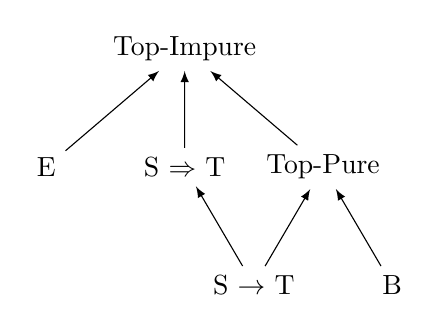
\begin{tikzpicture}[sibling distance=5em,
  every node/.style = {align=center},
  edge from parent/.style={draw,latex-}]
  \node {Top-Impure}
  child { node {E} }
  child { node (free) {S $\Rightarrow$ T} }
  child { node {Top-Pure}
    child { node (stoic) {S $\to$ T} }
    child { node {B} } };
  \path [draw, -latex] (stoic) -- (free);
\end{tikzpicture}

\caption{Subtyping: Top-Pure and Top-Impure}
\label{fig:stlc-impure-subtyping-tree}
\end{figure}

The second possibility is to keep the elegance of the type system and
changes the evaluation rules. We know that all terms of the type Top
are equivalent, because we can do nothing with a term of type Top. It
implies we can substitute them arbitrarily without changing the
meaning of the term. This observation inspires us to introduce a
\emph{top} value and change the standard E-AppAbs rule to two
evaluation rules as follows:

\infrule[E-AppAbs1]
{ T \neq Top }
{ (\lambda x:T.t_1) v_2 \longrightarrow [x \mapsto v_2]t_1 }

\infrule[E-AppAbs2]
{ T = Top }
{ (\lambda x:T.t_1) v_2 \longrightarrow [x \mapsto top]t_1 }

The two rules have the effect that if a function takes a parameter of
type Top, then when called it will drop the parameter and replace it
with the \emph{top} value. We follow this approach in the formulation
and the full definition is presented in
Figure~\ref{fig:stlc-impure-definition}.

\begin{figure}
\begin{framed}

% multi-column separator
\setlength{\columnseprule}{0.4pt}
\begin{multicols}{2}

\textbf{Syntax}

\begin{tabu} to \linewidth {l l l X[r]}
  t   & ::= &                    & terms:               \\
      &     & \colorbox{shade}{top} & top value            \\
      &     & x                  & variable             \\
      &     & $\lambda$ x:T.t    & abstraction          \\
      &     & t t                & application          \\
\\
  v   & ::= &                    & values:              \\
      &     & $\lambda$ x:T.t    & abstraction value    \\
      &     & x                  & variable value       \\
      &     & \colorbox{shade}{top}  & top value            \\
\\
  T   & ::= &                    & types:               \\
      &     & \colorbox{shade}{Top}  & top type             \\
      &     & B                  & basic type           \\
      &     & E                  & capability type      \\
      &     & T $\to$ T          & type of stoic funs       \\
      &     & \colorbox{shade}{T $\Rightarrow$ T} & type of free funs   \\
\end{tabu}

% \hfill\\
\vspace{0.1em}

\textbf{Evaluation} \hfill \framebox[1.2\width][r]{$t \longrightarrow t'$}

\infrule[E-App1]
{ t_1 \longrightarrow t'_1 }
{ t_1 \; t_2 \longrightarrow t'_1 \; t_2 }

\infrule[E-App2]
{ t_2 \longrightarrow t'_2 }
{ v_1 \; t_2 \longrightarrow v_1 \; t'_2 }

\infrule[E-AppAbs1]
{ \colorbox{shade}{$T \neq Top$} }
{ \colorbox{shade}{$(\lambda x:T.t_1) \; v_2 \longrightarrow [x \mapsto v_2]t_1$} }

\infrule[E-AppAbs2]
{ \colorbox{shade}{$T = Top$} }
{ \colorbox{shade}{$(\lambda x:T.t_1) \; v_2 \longrightarrow [x \mapsto top]t_1$} }

\textbf{Pure Environment}

\begin{center}
\begin{tabular}{l c l}
pure($\varnothing$)                   & = &   $\varnothing$ \\
pure($\Gamma$, x: E)                  & = &  pure($\Gamma$) \\
\rowcolor{gray!40}
pure($\Gamma$, x: S $\Rightarrow$ T)  & = &  pure($\Gamma$) \\
pure($\Gamma$, x: T)                  & = &  pure($\Gamma$), x: T     \\
\end{tabular}
\end{center}

\columnbreak

\textbf{Typing}  \hfill \framebox[1.2\width][r]{$\Gamma \vdash x : T$}

\infax[T-Top]{ \colorbox{shade}{$\Gamma \vdash top : Top$} }

\infrule[T-Var]
{ x: T \in \Gamma }
{ \Gamma \vdash x : T }

\infrule[T-Abs1]
{ pure(\Gamma),\; x: S \vdash t_2 : T }
{ \Gamma \vdash \lambda x:S.t_2 : S \to T }

\infrule[T-Abs2]
{  \colorbox{shade}{$\Gamma,\; x: S \vdash t_2 : T$} }
{  \colorbox{shade}{$\Gamma \vdash \lambda x:S.t_2 : S \Rightarrow T$} }

\infrule[T-App]
{ \Gamma \vdash t_1 : S \to T \andalso \Gamma \vdash t_2 : S }
{ \Gamma \vdash t_1 \; t_2 : T }

\infrule[T-Sub]
{  \colorbox{shade}{$\Gamma \vdash t : S \andalso S <: T$} }
{  \colorbox{shade}{$\Gamma \vdash t : T$} }

\colorbox{shade}{\textbf{Subtyping}}  \hfill \framebox[1.2\width][r]{$S <: T$}

\infax[S-Top]{ T <: Top }

\infax[S-Refl]{ T <: T }

\infrule[S-Trans]
{ S <: U \andalso U <: T }
{ S <: T }

\infrule[S-Degen]
{ S \to T }
{ S \Rightarrow T }

\infrule[S-Fun1]
{ S1 <: S2 \andalso T2 <: T1 }
{ S2 \to T2 <: S1 \to T1 }

\infrule[S-Fun2]
{ S1 <: S2 \andalso T2 <: T1 }
{ S2 \Rightarrow T2 <: S1 \Rightarrow T1 }

\hfill\\

\end{multicols}
\end{framed}

\caption{System STLC-Impure}
\label{fig:stlc-impure-definition}
\end{figure}

\subsection{Soundness}

We proved both progress and preservation in Coq based on the
locally-nameless representation.

\begin{theorem}[Progress]
If $\varnothing \vdash t : T$, then either $t$ is a value or there is some
$t'$ with $t \longrightarrow t'$.
\end{theorem}

\begin{theorem}[Preservation]
If $\Gamma \vdash t : T$, and $t \longrightarrow t'$, then $\Gamma
\vdash t' : T$.
\end{theorem}

As you can imagine, now we need two different substitution lemmas in
the proof of perservation, corresponding to the two reduction rules.

\begin{lemma}[Subsitution-Not-Top]
  If $\Gamma,\; x:S \vdash t : T$, $S \neq Top$, s is a value and
  $\Gamma \vdash s : S$, then $\Gamma \vdash [x \mapsto s]t : T$.
\end{lemma}

\begin{lemma}[Subsitution-Top]
  If $\Gamma,\; x:Top \vdash t : T$, then $\Gamma \vdash [x \mapsto top]t : T$.
\end{lemma}

\subsection{Effect Safety}

We follow the same approach as the system STLC-Pure in formulation of
effect safety. The formulation is an extension of the definition of
capsafe/caprod in STLC-Pure with free function types.

\subsubsection{Formulation}

With the presence of free functions, the previous formulation of
effect safety is not enough. We not only need to ensure that it's
impossible to construct a term of the capability type in healthy
environments, but also need to ensure only stoic functions can be
called in healthy environments. The two conditions together guarantee
that there cannot be actual side effects inside a pure stoic
function. Thus, we need two statements about effect safety.

\begin{definition}[Effect-Safety-1]
  If $\Gamma$ is healthy, there doesn't exist $t$ with
  $\Gamma \vdash t : E$.
\end{definition}

\begin{definition}[Effect-Safety-2]
  If $\Gamma$ is healthy and $\Gamma \vdash t_1 \; t_2 : T$, then
  there exists U, V such that $\Gamma \vdash t_1 : U \to V$.
\end{definition}

A tempting formulation of the second effect safety statement would be
that in a healthy environment it's impossible to construct a term of
free function type. However, this formulation has no hope to be
proved, as $S \to T$ is a subtype of $S \Rightarrow T$, any term that
can be typed as the former can also be typed as the latter.

Now let's consider how to define caprod/capsafe for free function
types. Our first attempt is to add following rule:

\infax[CP-Fun2]{ S \Rightarrow T \quad caprod }

With this rule, the type $(B \Rightarrow B) \to E$ is considered
capsafe, according to the CP-Fun1 rule. However, with a variable $f$
of this type in the healthy environment, together with another
variable $g$ of the capsafe type $B \to B$, it's possible to create
the term \emph{f g}, which is of the capability type. On ther other
hand, it doesn't make sense to take $S \Rightarrow T$ as capsafe, as
it would allow calling free functions in healthy environments,
which also breaks the effect safety.

This dilemma prompts us to reexamin the meaning of \emph{capsafe} and
\emph{caprod}. When these facilities were introduced in STLC-Pure, they
are formulated through the provability of the capability type E. From
the perspective of provability of E, $S \to T$ and $S \Rightarrow T$
don't make much difference. Thus, free functions types should be
formulated the same way as sotic function types. We tried this
approach, and it worked. The full formulation is presented in
Figure~\ref{fig:stlc-impure-healthy-definition}.

\begin{figure}[h]
\begin{framed}

% multi-column separator
\setlength{\columnseprule}{0.4pt}
\begin{multicols}{2}

\textbf{Capsafe}

\infax[CS-Base]
{ B \quad \text{capsafe} }

\infrule[CS-Fun1]
{ S \quad caprod }
{ S \to T \quad \text{capsafe} }

\infrule[CS-Fun2]
{ T \quad \text{capsafe} }
{ S \to T \quad \text{capsafe} }

\infrule[CS-Fun3]
{ \colorbox{shade}{$S \quad caprod$} }
{ \colorbox{shade}{$S \Rightarrow T \quad \text{capsafe}$} }

\infrule[CS-Fun4]
{ \colorbox{shade}{$T \quad \text{capsafe}$} }
{ \colorbox{shade}{$S \Rightarrow T \quad \text{capsafe}$} }

\columnbreak

\textbf{Caprod}

\infax[CP-Eff]
{ E \quad caprod }

\infrule[CP-Fun1]
{ S \; \text{capsafe} \andalso T \; caprod }
{ S \to T \quad caprod }

\infrule[CP-Fun2]
{ \colorbox{shade}{$S \; \text{capsafe} \andalso T \; caprod$} }
{ \colorbox{shade}{$S \Rightarrow T \quad caprod$} }

\textbf{Healthy}

\infax[H-Empty]
{ \varnothing \quad caprod }

\infrule[H-Var]
{ G \; healthy \andalso T \; \text{capsafe} }
{ G, \; x:T \quad healthy }

\hfill\\

\end{multicols}
\end{framed}

\caption{System STLC-Impure Healthy Environment}
\label{fig:stlc-impure-healthy-definition}
\end{figure}

A consequence of this definition that a healthy environment is no
longer pure. Conceptually speaking, a healthy environment should
always be a subset of pure environment. However, this is not a
problem. We can define
$healthy' \; E := healthy \; E \wedge pure \; E = E$. Effect safety
proved only assuming \emph{healthy} also holds for $healthy'$. But
what's the purpose of defining such a weaker concept of
\emph{healthy}? The answer is that it makes the first statement of
effect safety simpler. As we'll see, the proof of the first statement
of effect safety only depends on \emph{healthy}, while the second
depends on \emph{healthy'}.

Another question is, how can we be sure that the new CP-Fun2 rule only
reject non-inhabitable types in pure environments? As before, we only
provide informal arguments here. In fact, the type $B \Rightarrow E$
rejected by CP-Fun2 is inhabitable, as free functions can capture
any capabilities in scope. However, as all free function types
like $S \Rightarrow T$ are already removed from the pure environment,
it's fair enough to remove some of them from the healthy environment.

The justification for CP-Fun1 is as before - given a proof from which
E can't be proved, we can't transform it to a proof capable of proving
E, together with a group of premises incapable of proving E.

\subsubsection{Proof}

The proof of the first statement of effect safety is almost the same
as in STLC-Pure. However, we need to add a \emph{Capsafe-Sub} lemma.
The first effect safety statement follows immediately from the lemma
\emph{Healthy-Capsafe}.

\begin{lemma}[Capsafe-Not-Caprod]
 If type T is capsafe, then T is not caprod.
\end{lemma}

\begin{lemma}[Capsafe-Or-Caprod]
 For any T, T is either capsafe or caprod.
\end{lemma}

\begin{lemma}[Capsafe-Sub]
 If S is capsafe and $S <: T$, then T is capsafe.
\end{lemma}

\begin{lemma}[Healthy-Capsafe]
  If $\Gamma$ is healthy and $\Gamma \vdash t : T$, then T is capsafe.
\end{lemma}

\begin{theorem}[Effect-Safety-1]
  If $\Gamma$ is healhty, then there doesn't exist term $t$ with
  $\Gamma \vdash t : E$.
\end{theorem}

The proof of the second effect safety statement is hopeless, unless we
assume four well-founded axioms listed in
Figure~\ref{fig:stlc-impure-axioms}. These axioms can only be proved if
$\Gamma$ is empty. Otherwise, if $t$ is a variable, we can do nothing.

\begin{figure}[h]
\begin{framed}

% multi-column separator
% \setlength{\columnseprule}{0.4pt}
\begin{multicols}{2}

\infrule[Ax-Base]
{ \Gamma \vdash t : B \to S \Rightarrow T }
{ \Gamma \vdash t : B \to S \to T }

\hfill\\

\infrule[Ax-Top]
{ \Gamma \vdash t : Top \to S \Rightarrow T }
{ \Gamma \vdash t : Top \to S \to T }

\hfill\\

\infrule[Ax-Stoic]
{ \Gamma \vdash t : (U \to V) \to S \Rightarrow T }
{ \Gamma \vdash t : (U \to V) \to S \to T }

\hfill\\

\infrule[Ax-Poly]
{ \Gamma \vdash t_2 : U \to V \\
  \Gamma \vdash t_1 : (U \Rightarrow V) \to S \Rightarrow T }
{ \Gamma \vdash t_1 \; t_2 : S \to T }

\end{multicols}
\end{framed}

\caption{System STLC-Impure Axioms}
\label{fig:stlc-impure-axioms}
\end{figure}

The justification for the axiom \textsc{Ax-Base} is as
follows. Suppose $t = \lambda x:B. \; \lambda y:S. \; t_1$ and
$\Gamma \vdash t : B \to S \Rightarrow T$. The typing rule for $t$
should be the typing rule for stoic functions:

\infrule[Step-1]
{ pure(\Gamma),\; x: B \vdash \lambda y:S. \; t_1 : S \Rightarrow T }
{ \Gamma \vdash \lambda x:B. \lambda y:S. \; t_1 : B \to S \Rightarrow T }

Then what's the rule used in the typing of $\lambda y:S. \; t_1$? If it's
first typed as $S \to T$ and then subsumed to $S \Rightarrow T$, then
we are done. Otherwise, $\lambda y:S. \; t_1$ is typed using the rule of
free functions:

\infrule[Step-2]
{ pure(\Gamma),\; x: B,\; y:S \vdash t_1 : T }
{ pure(\Gamma),\; x: B \vdash \lambda y:S. \; t_1 : S \Rightarrow T }

According to the definition of \emph{pure}, we know that following two
equations holds:

\begin{itemize}
\item $pure(pure(\Gamma)) = pure(\Gamma)$
\item $pure(\Gamma, x:B) = pure(\Gamma), x:B$
\end{itemize}

From the equations above, we have can get following equation:

\begin{center}
  $pure(pure(\Gamma),\; x: B) = pure(\Gamma),\; x: B$
\end{center}

If we substitute the equation in Step-2, we get exactly the
precondition for typing stoic functions. Thus $\lambda y:S.t_2$ can be
typed as stoic function:

\infrule[Step-2']
{ pure(pure(\Gamma),\; x: B),\; y:S \vdash t_1 : T }
{ pure(\Gamma),\; x: B \vdash \lambda y:S. \; t_1 : S \to T }

Because we know $\lambda y:S. \; t_1$ is typed as $S \to T$, so we can
update Step-1 as following:

\infrule[Step-1']
{ pure(\Gamma),\; x: B \vdash \lambda y:S. \; t_1 : S \to T }
{ \Gamma \vdash \lambda x:B. \lambda y:S. \; t_1 : B \to S \to T }

Put all the steps together, we've inferred
$\Gamma \vdash t : B \to S \to T$ from the fact
$\Gamma \vdash t : B \to S \Rightarrow T$. That's the justification
for the \textsc{Ax-Base} rule. The justifications for \textsc{Ax-Top}
and \textsc{Ax-Stoic} are similar. The axiom \textsc{Ax-Poly} is an
interesting one, which deserves a separate section.

Assuming the axioms above, it's straight-forward to prove a lemma
\emph{Healthy-Pure-Stoic}, and the second statement of effect safety
follows immediately from the lemma.

\begin{lemma}[Healthy-Pure-Stoic]
  If $\Gamma$ is healthy and pure,  and $\Gamma \vdash t : S
  \Rightarrow T$, then $\Gamma \vdash t : S \to T$.
\end{lemma}

\begin{theorem}[Effect-Safety-2]
  If $\Gamma$ is healthy and pure, and $\Gamma \vdash t_1 \; t_2 :
  T$, then there exists U, V such that $\Gamma \vdash t_1 : U \to V$.
\end{theorem}

Note that unlike the proof of the first effect safety statement, the
proof of the second statement of effect safety assumes that $\Gamma$
is pure. This is due to the fact that \emph{healthy} no longer implies
\emph{pure}. Conceptually speaking, a healthy environment should
always be a subset of pure environment. To clear the worry of readers,
we can define $healthy' \; E := healthy \; E \wedge pure \; E = E$.
Effect safety proved only assuming the weaker \emph{healthy} also
holds for $healthy'$.

\subsubsection{Effect Polymorphism}

The axiom \textsc{Ax-Poly}, which we call \emph{effect polymorphism},
reflects some important property about capability-based effect
systems. Suppose following typing relation holds, what impure
variables can be captured by $t_1$?

\begin{center}
  $\Gamma \vdash \lambda f:U \Rightarrow V. \; \lambda y:S. \; t_1 : (U
  \Rightarrow V) \to S \Rightarrow T$.
\end{center}

As the functioin is stoic, the only impure variable can be captured is
$f$. Now, if we supply a stoic function as parameter to the function,
it has the same effect as saying that $f$ is $U \to V$. Thus in this
context, the function can be typed as $(U \to V) \to S \Rightarrow T$.
Now according to the \textsc{Ax-Stoic} axiom, the term can also be
typed as $(U \to V) \to S \to T$. Then according to the standard
\textsc{T-App} rule, we can get the type of the application is
$S \to T$. That's the justification for the axiom \textsc{Ax-Poly}.

Effect polymorphism is an advantage of capability-based effect systems
over monad-based effect systems. In Haskell, there is always the need
to maintain two copies of higher-order functions, as following code
snippet shows\footnote{From the slides of Ben Lippmeier,
  \emph{Witnessing Purity, Constancy and Mutability}, APLAS 2009}:

\begin{lstlisting}[language=Haskell]
  map :: (a -> b) -> List a -> List b
  map f xs
    = case xs of
        Nil -> Nil
        Cons x xs -> Cons (f x) (map f xs)

  mapIO :: (a -> IO b) -> List a -> IO (List b)
  mapIO f xs
    = case xs of
      Nil -> return Nil
      Cons x xs -> do x' <- f x
        xs' <- mapIO f xs
        return (Cons x' xs')
\end{lstlisting}

The non-monadic version and the monadic version of code are the same
in essence. It's a pity we have to duplicate the same code twice in
monad-based effect systems. In capability-based effect systems, we
only need to maintain one copy of the code:

\begin{lstlisting}[language=Scala]
  def map[A,B](f: A => B)(l: List[A]) = l match {
    case Nil => Nil
    case x::xs => f(x)::map(f)(l)
  }
\end{lstlisting}
% haskell two versions of map

The \emph{map} function above has the type
$(A \Rightarrow B) \to List[A] \Rightarrow List[B]$. Is \emph{map} a
pure function? It depends on how it's used. When supplied with a pure
function $f$ of type $A \to B$, \emph{map} has the type
$(A \to B) \to List [A] \to List[B]$, thus is pure. When supplied with
a function of type $A \Rightarrow B$ with side effects, \emph{map} is
impure. This is a good news for programmers in want of effect
polymorphism.
